%%%%%%%%%%%%%%%%%
% Modelo de relatório de Disciplina de MLP a partir da
% classe latex iiufrgs disponivel em http://github.com/schnorr/iiufrgs
%%%%%%%%%%%%%%%%%

%%%%%%%%%%%%%%%%%
% Definição do tipo / classe de documento e estilo usado
%%%%%%%%%%%%%%%%%
%
\documentclass[rel_mlp]{iiufrgs}

%%%%%%%%%%%%%%%%%
% Importação de pacotes
%%%%%%%%%%%%%%%%%
\usepackage[brazilian]{babel}	    % para texto escrito em pt-br
\usepackage[utf8]{inputenc}         % pacote para acentuação
\usepackage{graphicx}         	    % pacote para importar figuras
\usepackage[T1]{fontenc}            % pacote para conj. de caracteres correto
\usepackage{times}                  % pacote para usar fonte Adobe Times
\usepackage{enumerate}              % para lista de itens com letras
\usepackage{breakcites}
\usepackage{titlesec}
\usepackage{enumitem}
\usepackage{titletoc}               
\usepackage{listings}			    % para listagens de código-fonte
\usepackage{mathptmx}               % p/ usar fonte Adobe Times nas formulas matematicas
\usepackage{url}                    % para formatar URLs
%\usepackage{color}				    % para imagens e outras coisas coloridas
%\usepackage{fixltx2e}              % para subscript
%\usepackage{amsmath}               % para \epsilon e matemática
%\usepackage{amsfonts}
%\usepackage{setspace}			    % para mudar espaçamento dos parágrafos
%\usepackage[table,xcdraw]{xcolor}  % para tabelas coloridas
%\usepackage{longtable}             % para tabelas compridas (mais de uma página)
%\usepackage{float}
%\usepackage{booktabs}
%\usepackage{tabularx}
%\usepackage[breaklinks]{hyperref}

\usepackage[alf,abnt-emphasize=bf]{abntex2cite}	% pacote para usar citações abnt
\usepackage{verbatim}
%%%%%%%%%%%%%%
% Macros, ajustes e definições
%%%%%%%%%%%%%%
%

% define estilo de parágrafo para citação longa direta:
\newenvironment{citacao}{
    %\singlespacing
    %\footnotesize
    \small
    \begin{list}{}{
        \setlength{\leftmargin}{4.0cm}
        \setstretch{1}
        \setlength{\topsep}{1.2cm}
        \setlength{\listparindent}{\parindent}
    }
    \item[]}{\end{list}
}

% adiciona a fonte em figuras e tabelas
\newcommand{\fonte}[1]{\\Fonte: {#1}}

% Ative o seguinte caso alguma nota de rodapé fique muito longa e quebre entre múltiplas
% páginas
%\interfootnotelinepenalty=10000

%%%%%%%%%%%%%%
% Informações gerais                                   
%%%%%%%%%%%%%%

% título
\title{Projeto Inicial  do Trabalho Final para a Disciplina de MLP do Instituto de Informática da UFRGS} 

% autor
\author{Dexheimer}{André}
\author{Piscoya}{Gabriel}
\author{Wiebbelling}{Rodrigo}

% Professor orientador da disciplina
\advisor[Prof.~Dr.]{Mello Schnorr}{Lucas}

% Nome do(s) curso(s):
\course{Curso de Graduação em Ciência da Computa{\c{c}}{\~a}o e Engenharia de Computação}

% local da realização do trabalho 
\location{Porto Alegre}{RS} 

% data da entrega do trabalho (mês e ano)
\date{12}{2017}

% Palavras chave
\keyword{Tower Defence}
\keyword{Orientação a Objetos}
\keyword{Functional}
\keyword{C++}
\keyword{MLP}

%%%%%%%%%%%%%%
% Início do documento e elementos pré-textuais
%%%%%%%%%%%%%%

% Declara início do documento
\begin{document}

% inclui folha de rosto 
\maketitle      

\selectlanguage{brazilian}

% Sumario
\tableofcontents


\bibliographystyle{abntex2-alf}


%\bibliography{biblio} % arquivo que contém as referências (no formato bib). Colocar as suas 
%%%%%%%%%%%%%
% Aqui comeca o texto propriamente dito
%%%%%%%%%%%%%

%espaçamento entre parágrafos
%\setlength{\parskip}{6 pt}
%\setlength{\parskip}{6 pt}

%\selectlanguage{brazilian}


\chapter{Introdução} \label{intro}
Este capítulo tem o objetivo de descrever de forma sucinta a historia das linguagens de programação e os principais tópicos envolvidos na realização deste trabalho. Logo após, serão abordados os temas diretamente relacionados ao trabalho. 

\section{Historia das Linguagens de Programação}
As primeiras linguagens de programação eram simples códigos utilizados para automatizar processos nem sempre relacionadas à computação. Na década de 1940, com a criação do primeiro computador moderno, eram utilizados cartões perfurados para facilitar o processo de programação e diminuir a quantidade de erros introduzidos pelo programador. Não foi até meados de 1950 que surgiu a primeira linguagem de programação moderna: FORTRAN, criada por John Backus. Os seguintes anos foram frutíferos, vieram acompanhados de duas novas linguagens de programação: LISP - John McCarthy e COBOL - Grace Hopper.

No começo, todas as linguagens de programação somente permitiam a criação de programas monolíticos e careciam de recursos que facilitassem sua utilização. Somente no fim da década de 1970 que foram estabelecidos os principais paradigmas de programação conhecidos hoje em dia: imperativo, funcional e lógico.
Durante estes anos, surgiu o termo "Programação Estruturada", que visava restringir o uso de desvios incondicionais (GoTo) \cite{organick2014programming}.

Em 1980, foi criada C++, que combinava orientação a objetos e programação de sistemas, também foi introduzida uma mudança de pensamento na concepção de linguagens de programação, junto com o movimento RISC em arquitetura de computadores, despertou-se maior interesse no uso de compiladores para linguagens de alto nível.

Com a chegada da internet, sugiram as linguagens de scripting, que não são evolução direta de nenhuma linguagem já estabelecida anteriormente, e que foram concebidas com novas sintaxes e novas funções \cite{ceruzzi1998history}.

\section{Ambiente e Linguagem de Programação}
Como o objetivo do trabalho é aproximar os alunos das linguagens de programação modernas, optamos por escolher uma linguagem que seja amplamente usada na atualidade, também sabemos que ela deve ser multi paradigma, já que devemos implementar soluções utilizando dois paradigmas diferentes.
Pelos motivos citados previamente, escolhemos \textbf{C++}.

\section{Problema Abordado}
A intenção inicial foi a de resolver um problema que já fosse conhecido pelos integrantes do grupo e que despertasse o interesse de todos, portanto escolhemos \textbf {Tower Defence}.

\chapter{A Linguagem C++} \label{C++}

A linguagem de programação C++ foi criada por Bjarne Stroustrup nos anos de 1980, vindo a ter sua padronização ISO apenas 18 anos depois em 1998. Ela é uma linguagem compilada multi-paradigma, com suporte ao modelo imperativo, ao orientado a objetos, ao genérico, entre outros. Por causa disso, é de uso amplo entre as linguagens comerciais e acadêmicas.

\section{Algumas características do C++}

	\textbf{Operadores:} O C++ possui todo o conjunto de operadores do C, além de alguns implementados apenas no C++, que dizem respeito à conversão entre tipos, os quais que podem ser const\_cast, static\_cast, dynamic\_cast e reinterpret\_cast. Além disso, a linguagem possui sobrecarga de operadores, permitindo que um mesmo operador tenha mais do que 1 significado dependendo do contexto em que é utilizado.

	\textbf{	Pré-Processador:} antes da compilação propriamente dita, o C++ passa pelo seu pré-processador, gerando modificações léxicas que servem como entrada para a compilação.

	\textbf{Objetos:} O C++ tem suporte aos conceitos de orientação à objetos, permitindo a criação de classes que apresentam quatro características desses conceitos: abstração, encapsulamento, herança e polimorfismo. O encapsulamento permite proteger atributos e métodos do objeto, dessa forma  é possível que outros trechos do programa tenham acesso apenas aos métodos de interface com a classe.	A herança de classes permite que uma classe herde atributos e métodos de outra, podendo ser relacionado com a ideia de classes mãe e filha. O polimorfismo trata da capacidade de se utilizar um operador ou método de diferentes maneiras, facilitando a estendibilidade da classe.

	\textbf{	Tratamento de Exceções:} Erros podem ser tratados pelo sistema, permitindo que a aplicação se recupere de algum erro sem travar ou ter de ser fechada.

	\textbf{Espaço de Nomes:} Permite uma melhor organização das bibliotecas, de forma que cada uma pode criar o seu próprio espaço de nomes para que não existam conflitos.

\chapter{Tower Defence} \label{Tower Defence}
É um estilo de jogo de estratégia que consiste em defender uma determinada entidade de inimigos. No nosso jogo, a entidade em questão é uma torre que se encontra no centro da tela. Esta torre possui uma certa quantidade de vida, velocidade de ataque, penetração de armadura, dano e alcance de ataque. Tais características podem ser melhoradas e outras habilidades podem ser adquiridas por meio de compras com a unidade monetária do jogo, obtida matando os inimigos.

\section{Objetivo do jogo}
Defender a sua torre de ondas progressivamente maiores de inimigos progressivamente mais fortes.

\section{Os inimigos}
Eles têm como objetivo atacar a torre até que sua vida chegue a 0 pontos, surgem de pontos aleatórios nas bordas da tela e vão em direção a torre. Eles possuem atributos definidos pelo nível do jogo, como: velocidade de ataque e de movimento, poder de ataque, quantidade de vida e de defesa.
	Existem 3 classes de inimigos: a classe "Soldier" se trata de um soldado que anda a pé e possui apenas armas de curto alcance. Ele vai em direção ao centro da tela e somente danifica a torre ao chegar nela.
	A classe "Horseman" se comporta de maneira semelhante ao soldier, porém possui mais defesa, dano de ataque e velocidade de movimento.
	A classe "Archer" é a que mais se diferencia das outras pois consegue atacar a torre de longas distâncias, tendo em suas características algo que as outras classes não têm, a distância de ataque, que indica a distância da qual o inimigo deve estar da torre para poder atacá-la. 

\chapter{ Implementação Orientada a Objetos} \label{Implementação OO}
Na linguagem C++, o paradigma orientado a objetos é o mais conhecido, logo é o mais utilizado entre os programadores.
Serão introduzidos os conceitos principais abordados neste trabalho para depois realizar uma breve discução sobre quando e onde devem ser utilizados.
\section{Classes}
O propósito principal da programação em C++ é a acrescentar orientação a objetos à linguagem C. Classes são a característica principal da linguagem C++ que suporta orientação a objetos, também são chamadas de tipos definidos pelo usuário. A diferença das estruturas de dados presentes em C, as classes combinam a representação dos dados com métodos associados, formando assim uma unidade compacta. 
\bigbreak

\begin{figure}[htb]
    \centering
    \fbox{
        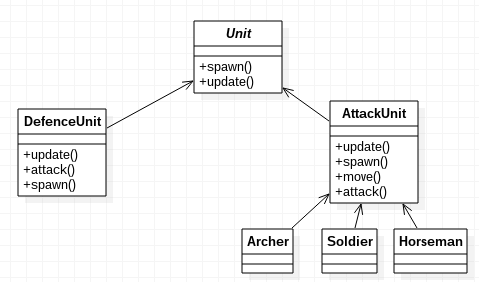
\includegraphics[width=10cm,height=7cm,keepaspectratio]{images/class_diagram.png}
    }
    \label{fig:figura1}
    \caption{Diagrama de Classes Simplificado.}
    %\fonte{xxxxxx}
\end{figure}


\subsection{Classes Abstratas}
As classes abstratas são um tipo de classes que agem como expressões de conceitos gerais das quais classes mais específicas podem ser derivadas. Não está permitido instanciar objetos de classes abstratas. 
Uma classe derivada de uma classe abstrata deve implementar o método virtual puro ou também será considerada uma classe abstrata.

\noindent {Métodos virtuais puros são declarados da seguinte forma:}
 \begin{itemize}
 \item virtual void pureVirtualFunction() = 0  
 \end{itemize}  	
A classe \textbf{Unit} é uma classe abstrata já que define metodos virtuáis puros que são implementados nas classes derivadas correspondentes( AttackUnit e DefenceUnit).
\subsection{Herança}
Herança é fundamental na programação orientada a objetos, já que fornece meios para promover a extensibilidade do codigo, reutilização e maior coerência lógica no modelo de implementação. As classes que são usadas para derivação são chamadas de classes base de uma classe derivada específica.Na herança a classe derivada contém os membros da classe base mais os novos mebros que sejam adicionados na declaração da classe derivada.
\noindent {Herança é declarada da seguinte forma:}
 \begin{itemize}
 \item class Derived :[virtual] [access-specifier] Base
 \{ \bigbreak
 	\hspace{1cm} // Member List		
	\bigbreak
 \};  
 \end{itemize}  	
\subsection{Herança Unica} 	
As classes tem apenas uma classe base, gerando assim uma árvore de derivação.

\begin{figure}[htb]
    \centering
    \fbox{
        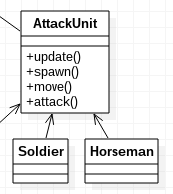
\includegraphics[width=8cm,height=5cm,keepaspectratio]{images/heranca_unica.png}
    }
    \label{fig:figura2}
    \caption{Herança Unica.}
    %\fonte{xxxxxx}
\end{figure}


\subsection{Herança Multipla} 	
As classes podem herdar de mais de uma classe base, gerando assim um grafo de derivação.
\noindent {Herança multipla apresenta diversos problemas de implementação:}
 \begin{itemize}
   \item Problema do Diamante: Uma classe D herda de duas classes B e C. B e C herdam de A. Os atributos de A serão duplicados em D gerando   assim conflitos e ambiguidades no momento do acesso. 
\begin{figure}[htb]
    \centering
    \fbox{
        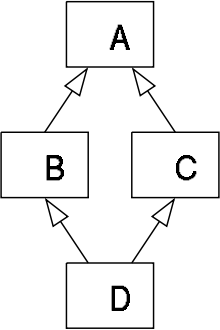
\includegraphics[width=8cm,height=5cm,keepaspectratio]{images/diamante.png}
    }
    \label{fig:figura3}
    \caption{Problema do Diamante.}
    %\fonte{xxxxxx}
\end{figure}
   
   
   
   Uma solução para este problema  é utilizar herança virtual nas classes B e C.
 \end{itemize}  	
 A planificação inicial foi feita de modo a evitar o uso de Herança Multipla.
 
 
 
\section{Encapsulamento} 
 
	O encapsulamento consiste em isolar atributos e métodos afim de progê-los de qualquer uso indevido, isto, junto com a devida documentação, favorece em muito a reusabilidade do código, uma vez que facilita sua correta instanciação.
	
	Na nossa implementação, fizemos com que quase, senão todos, os atributos das classes fossem protegidos, isto permite que eventuais classes que herdem destas ainda consigam utilizá-los. Aliando isso aos métodos de acesso (\textit{getters} e \textit{setters}), temos uma camada que torna mais difícil o assinalamento de dados inválidos ou inesperados a variáveis internas, assim tornando o código mais robusto e seguro.
	
 	No nosso código, o trecho onde essa propriede se torna mais visível é na classe \textit{Unit}, a qual possui dados sobre todas as unidades de ataque e de defesa presentes no jogo. Aqui, todas as variáveis são protegidas para que nenhum contexto de fora possa fazer alterações diretas. Isto se tornou importante não só para manter a integridade dos dados, mas também porque todos os atributos de ataque de defesa devem se manter consistentes com seus níveis já que, apenas assim, o sistema de \textit{upgrades} pode funcionar corretamente. Portanto, todas as alterações a esses atributos só podem ser feitas por meio dos métodos que levam em consideranção os seus valores base e seus níveis atuais.
 	
 	
 \section{Delegates}
 
 	Delegates consistem em uma maneira de generalizar tarefas que possuem diferentes rotinas e/ou entradas para um mesmo fim. No nosso código, encontramos dificuldades em implementar Delegates como normalmente são feitos em C++, com classes ou structs específicas para este fim. Portanto, tentamos utilizar caracteríscas desse modelo em algumas funções específicas. Os melhores exemplos disso a serem citados na nossa implementação desta etapa do trabalho estão na classe \textit{Unit} e dizem respeito ao sistema de \textit{upgrades}. 
 	
 	Esse sistema necessita de três informações básicas: o nível de um atributo, o seu valor base (inicial) e um coeficiente de aumento. Então juntamos estas três informações em três chamadas que realizam as seguintes operações sobre todos os atributos: consultar um valor, verificar e incrementar seu nível atual. Estas funções possuem em comum um parâmetro que consiste em uma \textit{enum} que define o nome de um dado (vida, armadura, dano de ataque, número de alvos, velocidade de ataque e alcance de ataque). Desta forma, cada função pode realizar seis ações diferentes, sendo uma para cada atributo.
 
 
 \section{Análise Crítica}
 
 \begin{center}
\begin{tabular}{ |c|c|p{80mm} } 
\hline
	\textbf{Critérios} & \textbf{Nota} & \textbf{Justificativas} \\
\hline
\textbf{Simplicidade} & 6 & Pode se tornar bastante complexo uma vez que é necessário administrar ponteiros para listas e alocação de memória. \\ 
\textbf{Ortogonalidade} & 6 & a \\ 
\textbf{Expressividade} & 5 & a \\ 
\textbf{Adequabilidade} & 9 & a \\
\textbf{Variedade de estruturas de controle} & 10 & a \\
\textbf{Mecanismos de definição de tipos} & 10 & a \\
\textbf{Suport a abstração de dados e de processos} & 10 & a \\
\textbf{Modelo de tipos} & 10 & a \\
\textbf{Portabilidade} & 10 & a \\
\textbf{Reusabilidade} & 10 & a \\
\textbf{Suporte e documentação} & 10 & a \\ 
\textbf{Tamanho de código} & 7 & a \\
\textbf{Generalidade} & 7 & a \\
\textbf{Eficiência e custo} & 10 & a \\

\hline
\end{tabular}
\end{center}
 
 
 
 
 
 
%%%%%%%%%%%
% Referências 
%%%%%%%%%%%

%\bibliographystyle{abnt}

%\bibliographystyle{abntex2-alf}

\bibliography{biblio} % arquivo que contém as referências (no formato bib). Colocar as suas lá (se tiver dúvida sobre como adicionar novas referências, usar o software JabRef ou Medley)

\begin{comment}

\noindent {\\\bf Se tiver alguma dúvida, veja os exemplos seguintes:}\\

\noindent {\bf \underbar{Monografia no todo}}\\

\noindent {\bf Livros e Anais de Congresso (Autor. Título. Edição. Local de Publicação: editora, ano de publicação).}\\

\noindent FURASTÉ, Pedro Augusto. {\bf Normas Técnicas para o Trabalho Científico}: explicitação das normas da ABNT. Porto Alegre: [s.n.], 2002. p. 49-56.

\noindent BRADLEY, N. {\bf The XML Companion}. 3${}^{rd}$ ed. Boston: Addison-Wesley, 2002.






\noindent {\bf \underbar{Norma}}\\

\noindent INSTITUTE OF ELECTRICAL AND ELECTRONIC ENGINEERING. {\bf IEEE 1003.1c-1995}: information technology -- portable operating system interface (POSIX), threads extension [C language]. New York, 1995.

\noindent ~

\noindent {\bf \underbar{Observações}}\\

\begin{comment}
Quando existirem mais de três autores, indica-se apenas o primeiro, acrescentando-se a expressão et al. Ex.: URANI, A. et al. Em casos em que a menção dos nomes for indispensável para certificar a autoria é facultado indicar todos os nomes.

Em caso de autoria desconhecida, a entrada é feita pelo título. Ex.: DIAGNÓSTICO do Setor Editorial Brasileiro. São Paulo: Câmara Brasileira do Livro, 1993.

Quando houver uma indicação de edição, esta deve ser transcrita, utilizando-se abreviaturas dos numerais ordinais e da palavra edição, ambas na forma adotada na língua do documento.

Ex.: SCHAM, D. {\bf Schawm's Outline of Theory and Problems}. 5${}^{th}$ ed. New York: Schawm Publishing, 1956.

PEDROSA, I. {\bf Da Cor a Cor Inexistente}. 6. ed. Rio de Janeiro: L. Cristiano, 1995.

Não sendo possível determinar o local (cidade) de publicação, utiliza-se à expressão sine loco, abreviada, entre colchetes [S.l.].

Quando a editora não puder ser indicada, deve-se indicar a expressão sine nomine, abreviada, entre colchetes [s.n].

Quando o local e a editora não puderem ser identificados, utilizam-se [S.l.:s.n].
\end{comment}

\end{document}

